\chapter{Quit Complaining Completely}

Some bad habits look ugly from the beginning. Laziness, dishonesty, vanity, and greed are easy to name, even when they are hard to quit.

Complaint is more dangerous because it often feels justified.

A person complains after being treated unfairly. He complains because a plan failed, because a colleague disappointed him, because the economy is bad, because the family is difficult, because the school is poor, because the market is irrational, because the world is not arranged as it should be. Each sentence may contain some truth. That is exactly why the habit survives. Complaint borrows truth from reality, then uses that truth to steal attention from action.

The habit to quit completely is this:

\begin{quote}
Complaint.
\end{quote}

Not every description of a problem is complaint. A clear report can be useful: what happened, what it costs, what must change, who should act, by when. Complaint is different. Complaint circles the wound without treatment. It demands sympathy more than solution. It spends time proving pain, then leaves the problem where it was.

For a person walking toward wealth freedom, this is not a small matter. Attention is the first capital. Time is nonrenewable. Agency is fragile. Complaint consumes all three.

\section*{A Man Who Did Not Complain}

One of the strongest lessons can come from someone who never announces that he is teaching.

When I was young, I knew a man named Jin Guang. After I failed the college entrance exam the first time, I spent another year preparing, and finally entered a university I did not like. Around the end of my first year, during a summer visit home, I met Jin Guang on a bright afternoon. He had already become a contractor in the early wave of real estate fever.

It was 1992. China was changing fast. People who sensed the shift were borrowing money, starting businesses, chasing projects, and stepping into risks they did not fully understand. Contractors looked especially impressive. Jin Guang was short, wore jeans, had a close haircut, and carried one of those large early mobile phones that looked glamorous at the time and absurd later.

We walked to the river and sat on the embankment for an afternoon.

I knew his situation was not easy. He had borrowed heavily. He was young. He lacked experience. Money was trapped in projects. Older and sharper people had surrounded him. There were delays, debts, traps, and pressures.

Yet all afternoon he talked about interesting things. He laughed. He told stories. He did not mention his hardship. Not once.

At first I thought of asking about his troubles, but I quickly saw the uselessness of my concern. I had no ability to solve his problems. My sympathy would have been only a performance. Perhaps he was proud. Perhaps he simply had a better instinct. Whatever the reason, his refusal to complain entered me deeply.

Many years later, I met him again by accident on a train to Shenyang. By then I had graduated, worked for two years, and was preparing to study abroad. Jin Guang had not become the successful contractor people imagined. He had debts and years of trouble behind him. He was on his way to Russia to find a new path.

But when I saw him, it felt as if no time had passed. Same smile, same brightness, same easy manner. The large phone had become a thinner Nokia. The rest was unchanged. We talked through the night. Again, there was no complaint. No bitterness. No list of people who had wronged him. No display of suffering.

When we got off the train, he waved and disappeared into the crowd. I never saw him again.

For years afterward, when people asked how I became determined not to complain, I thought of him. He never told me a principle. His existence was the principle.

Some friends comfort you when you complain. Such friends may be kind, and kindness should be valued. But there is another kind of friend, rarer and more powerful: the person whose example makes complaint feel unnecessary. Around such a person, you remember that difficulty and dignity can coexist.

\section*{Complaint Is Contagious}

The opposite is also true.

After that train trip, I went to Korea. The next fourteen months became one of the darkest periods of my life, even though they were also among the most intense learning periods I ever had. I read heavily. I encountered important books. On paper, the time should have been fruitful.

Only later did I understand one reason it felt so dark: almost everyone around me complained constantly.

The larger environment was anxious. The Asian financial crisis had hit Korea hard. News reports were full of bankruptcies, suicides, ruined families, and fear. In the university, the small group of Chinese students often gathered and, within minutes, began to complain. They complained about Korea, China, money, school, teachers, classmates, politics, food, weather, and whoever was absent from the room. The words changed; the structure did not.

A complaining group creates its own weather. Everyone breathes it. Even if you say little, you inhale the pattern.

Years later, after returning to China, I met one of those classmates for a meal. He began again: complaint after complaint, a familiar flood. Then I noticed something frightening. I had started to complain too. The language came out naturally, as if an old program had been reactivated.

I paid the bill, politely ended the meeting, and decided not to continue those relationships.

Complaint spreads quietly. In the early stage, symptoms are hard to notice. By the time you realize your own speech has changed, the habit may already have settled into your mind.

This is why environment matters. Earlier chapters discussed the living world, and how the world responds to your stance. Complaint is one of the most direct ways to make your world worse. It does not merely describe an ugly world. It helps produce one, by training your attention to search for ugliness and by inviting others to do the same.

\section*{The Decision Rule}

The antidote is not forced cheerfulness. Some things are genuinely difficult. Some people are unfair. Some systems are badly designed. Some losses are real. Wealth freedom does not require pretending that pain is pleasure.

It requires a cleaner decision rule:

\begin{quote}
If a problem can be solved, solve it. If it cannot be solved, endure it. In neither case is complaint useful.
\end{quote}

This rule sounds simple because it is simple. Its difficulty lies in practice.

\begin{center}
\begin{tabular}{p{0.28\linewidth}p{0.52\linewidth}}
\hline
Situation & Proper use of attention \\
\hline
Can change it & Define the next action and act. \\
Cannot change it now & Build the strength, resources, or patience to bear it. \\
Can change it later & Train, save, study, negotiate, or prepare. \\
Should not remain in it & Plan an exit instead of rehearsing resentment. \\
\hline
\end{tabular}
\end{center}

Complaint usually appears before this classification. It avoids the hard question: which part belongs to ability, and which part belongs to endurance?

When you complain about work, ask what ability is missing. Is it communication, skill, bargaining power, savings, reputation, leverage, or the courage to leave? When you complain about family, ask what boundary, patience, money, independence, or emotional capacity is missing. When you complain about society, markets, or luck, ask what can actually be changed by you, and what must be included in the cost of living.

The useful question is not, ``Am I right to be upset?'' Often you are. The useful question is:

\begin{quote}
What does this complaint reveal about my current lack of ability or lack of endurance?
\end{quote}

That question hurts, but it returns control.

\section*{The Pop-Up Window}

A practical habit helps: count complaints.

Keep a small record. Each time you complain, mark it down. Do not write an essay. A short note is enough: time, topic, trigger. The act of recording becomes a small pop-up window in the mind.

\begin{center}
\begin{adjustbox}{max width=\linewidth}
\begin{tikzpicture}[
  box/.style={draw, rounded corners=2pt, align=center, minimum width=2.65cm, minimum height=0.82cm},
  arrow/.style={->, thick}
]
\node[box] (trigger) {Trigger};
\node[box, right=0.45cm of trigger] (urge) {Urge to\\complain};
\node[box, right=0.45cm of urge] (popup) {Notice\\and record};
\node[box, below=0.72cm of popup] (choice) {Solve or\\endure};
\draw[arrow] (trigger) -- (urge);
\draw[arrow] (urge) -- (popup);
\draw[arrow] (popup) -- (choice);
\end{tikzpicture}
\end{adjustbox}
\end{center}

At first the number may be embarrassing. That is useful. The embarrassment is data. Soon the count often falls, not because life has become easier, but because awareness interrupts the automatic script.

When you fail and complain again, do not add another complaint about your complaint. Record it. Later, ask three questions:

\begin{enumerate}
\item What did I complain about most often?
\item What weakness, dependency, fear, or unmet need does it reveal?
\item If the matter is beyond my present and future control, what must I build in order to bear it with dignity?
\end{enumerate}

This is metacognition in plain clothes. The mind watches the mind before the habit takes over.

If someone else reminds you that you are complaining, do not resist too quickly. The first reaction may be irritation, because complaint wants protection. Treat the reminder as an alarm. Wake up first. Defend yourself later only if defense is truly needed.

\section*{Speech Rebuilds the Brain}

Complaint is not harmless speech. Speech trains identity.

When people complain, they often begin by reporting pain. Then they add detail. Then they dramatize. They need sympathy, so they unconsciously make the story heavier. They become more vivid, more wounded, more trapped. The listener's attention rewards the performance. The speaker then performs the role more strongly.

After enough repetition, the role stops feeling like a role.

A person who repeatedly describes himself as unlucky begins to notice lucklessness everywhere. A person who repeatedly describes himself as exploited begins to see every request as exploitation. A person who repeatedly describes himself as helpless begins to lose the impulse to struggle.

This is the true cost of complaint. It is not only that it wastes time. It is not only that it exposes incapacity. Its deepest harm is that it slowly persuades you to stop fighting.

In ordinary times, discouragement is human. No one is made of iron. But in adversity, and especially at decisive moments, the habit of giving up becomes fatal. Complaint rehearses that surrender before the decisive moment arrives.

For wealth freedom, this is especially costly. The road requires long periods in which results lag behind effort. Skills take time to compound. Capital takes time to grow. Reputation takes time to form. Investment demands tolerance of cycles: growth, peak, recession, trough, recovery. A person who complains at every trough may exit precisely when endurance is most valuable.

\begin{center}
\begin{adjustbox}{max width=\linewidth}
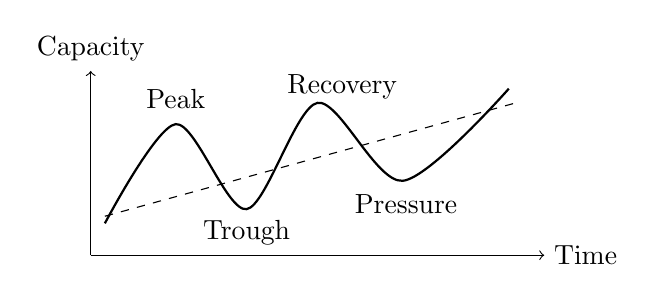
\begin{tikzpicture}[scale=0.9]
\draw[->] (0,0) -- (6.4,0) node[right] {Time};
\draw[->] (0,0) -- (0,2.6) node[above] {Capacity};
\draw[thick] plot[smooth] coordinates {(0.2,0.45) (1.2,1.85) (2.2,0.65) (3.2,2.15) (4.4,1.05) (5.9,2.35)};
\draw[dashed] (0.2,0.55) -- (6.0,2.15);
\node[align=center] at (1.2,2.2) {Peak};
\node[align=center] at (2.2,0.32) {Trough};
\node[align=center] at (3.55,2.38) {Recovery};
\node[align=center] at (4.45,0.72) {Pressure};
\end{tikzpicture}
\end{adjustbox}
\end{center}

The line of growth is not smooth. Complaint mistakes every downward swing for proof that effort is meaningless. Discipline sees the same swing and asks what should be learned, protected, or continued.

\section*{Choosing People}

After I decided to stop complaining, the principle became one of my most important standards for choosing friends.

This may sound severe, but it is practical. A person's language becomes part of your environment. If someone complains constantly, he is not merely describing his life to you. He is asking you to live inside his interpretation of life. If you accept the invitation often enough, your own interpretation changes.

This does not mean abandoning people in pain. There is a difference between helping a friend through a hard period and becoming an audience for a permanent habit. Compassion should not require the destruction of attention.

The closest relationships need special care. Family members and intimate friends often tolerate our complaint because they love us. Their tolerance can make us careless. Precisely because they are close, we should restrain ourselves more, not less. To dump repeated complaint on someone who cannot easily leave is a quiet form of unfairness.

Use a simple distinction:

\begin{center}
\begin{tabular}{p{0.35\linewidth}p{0.45\linewidth}}
\hline
Useful speech & Complaint \\
\hline
Names the problem clearly. & Repeats the injury endlessly. \\
Seeks action, decision, or comfort once. & Seeks sympathy as a habit. \\
Leaves room for responsibility. & Protects helplessness. \\
Ends with a next step or acceptance. & Ends where it began. \\
\hline
\end{tabular}
\end{center}

If a conversation cannot move toward action, boundary, learning, repair, or acceptance, it is likely becoming complaint.

\section*{Recognition Is a Bonus}

Many complaints are disguised demands for recognition.

``They do not understand me.''

``No one appreciates what I did.''

``Why does he get credit?''

``Why am I treated this way?''

Sometimes these complaints point to real problems. Credit matters. Fairness matters. Negotiation matters. A person should not romanticize being ignored.

But recognition is dangerous when treated as oxygen. If you cannot act without applause, then other people own your emotional engine. Better to treat recognition as an extra gift. Welcome it when it comes. Do not make it the condition for doing what is right, useful, or necessary.

This adjustment saves enormous attention. Instead of arguing endlessly about who is right, who noticed, who praised, and who failed to praise, you can return to the work itself.

Complaint tends to obsess over correctness. Freedom tends to ask for a way forward.

\begin{quote}
To remain tangled in right and wrong is to live tangled. To search for a way out is to live more freely.
\end{quote}

\section*{The Real Target}

When we complain about life, the hidden target is often ourselves.

We are dissatisfied with our weakness, but we describe it as dissatisfaction with the world. We are angry at our dependency, but we describe it as anger at other people. We are ashamed of our lack of options, but we describe it as proof that options do not exist.

This is why quitting complaint feels uncomfortable. It removes a shelter. Once the words stop, the remaining facts become visible.

But visibility is the beginning of power.

A person who stops complaining still has problems. He may still be poor, tired, wronged, behind, anxious, or unprepared. The difference is that his attention is no longer leaking through language. It can be gathered and spent.

The practice is severe and small:

\begin{enumerate}
\item Stop saying the complaint aloud.
\item Record each failure without drama.
\item Identify the missing ability.
\item Improve what can be improved.
\item Endure what cannot yet be changed.
\item Distance yourself, where possible, from chronic complaint.
\end{enumerate}

This is not positive thinking. It is resource protection.

The road to wealth freedom asks a person to become a better allocator: of money, time, effort, trust, risk, and attention. Complaint is bad allocation at the level of speech. It pays attention to pain without buying capacity. It spends emotion without purchasing clarity. It turns hardship into identity instead of material for growth.

Cherish life. Stay away from complaint, especially your own.
